\chapter{Experimental results with spatio-angular microscope}
\label{sec:results}
\begin{summary}
  Here I describe some of our experiments that demonstrate the
  functioning of our spatio-angular microscope prototype.

  In the first experiment, I use total internal reflection which
  prevents high angles from reaching the sample when the refractive
  index of the embedding medium is lower than that of the
  immersion medium. This allows to show in a simple way that the angular
  illumination control works.

  In the second experiment, we measure the three-dimensional light
  distribution in the sample by bleaching a fluorescent gel layer.

  Then I describe another experiment, that replicates the problem of
  imaging live specimens. The task is to localize three-dimensionally
  distributed beads and then image them individually using an
  optimized excitation light distribution.
\end{summary}

\section{Measuring acceptance angle for three different embedding
  media}
As one of the first attempts to use the spatio-angular illumination
system, I devised an experiment to determine the acceptance angle of a
microscope objective as a function of the embedding medium.

\begin{figure}[htbp]
  \centering
  \svginput{1}{tirf-exp}
  \caption{A fluorescent plane on a slide is embedded in oil, water or
    air. The thickness of the embedding medium is approximately
    $\unit[5]{\mu m}$. The focal plane SLM illuminates a disk with
    $\unit[30]{\mu m}$ diameter while a window of $15\times 15$ pixels
    is scanned over the MMA. The window corresponds to a square with
    $\unit[0.45]{mm}$ on the side as opposed to \unit[7.2]{mm} pupil
    diameter.  The red numbers indicate the diameter of the bright
    circle in pixels of the pupil plane SLM.
% 200 px diameter on LCoS
% 15x15 px full diameter is D=2*(R=f*NA) f=164.5/63=2.61  NA=1.38
% D=3.6mm -> D/256*15 = 210 um
% measuring fwhm in cross section:
% 241 or 244 px in oil
% 217 or 228 px in water
% 155 or 166 px air 
% measuring visible edge by drawing a circle in Fiji
% 270 in oil
% 237 in water
% 173 in air
% (%i2) 1.33/1.52;
% (%o2)                                0.875
% (%i3) 1/1.52;
% (%o3)                          .6578947368421053
% (%i8) 237/270,numer;
% (%o8)                          .8777777777777778
% (%i9) 173/270,numer;
% (%o9)                          .6407407407407407
% (%i11) ((7/270)+(7/237))*.8777777;
% (%o11)                        .04868312325832162
% (%i12) ((7/270)+(7/173))*.640740740740;
% (%o12)                        .04253772290804411
% (%i13) 
  }
  \label{fig:tirf-exp}
\end{figure}

For the measurement, a thin layer of fluorophores was applied with a
marker pen (Stanger, yellow-green) on three microscope slides. 
After drying, a drop of a liquid
embedding medium was added to two of the samples (immersion oil
($n=1.52$) and water ($n=1.33$)). Then cover slips were added to all
three samples and sealed with nail polish.

During \cma{scan pupil plane SLM} the measurement, the focal plane SLM
projected a disk with $\unit[30]{\mu m}$ diameter on the fluorescent
plane. The illumination angle was varied by stepping a window of
$15\times 15$ pixels (equivalent to 1/17th of the pupil diameter) over
the pupil plane SLM.

For each angle, the sum of all fluorescence light reaching the camera
is recorded. The fluorescence intensity for each window position on
the pupil plane SLM are depicted in the three images in
\figref{fig:tirf-exp}.  These images contain a bright disk whose
diameter $d_\textrm{crit}$ is growing with the index of the embedding
medium. The center of the disk corresponds to the optical axis of the
objective.  Points in the interior of the circle have an almost
constant intensity (residual fluctuations can be attributed to
non-uniformity of the illumination of the pupil plane SLM). For oil
immersion, the measured diameter of the disk corresponds to the
diameter of the pupil which is:
\begin{align}
  d^\textrm{(theory)}_\textrm{pupil} &=
  2\textrm{NA}\cdot f_\textrm{obj} =\unit[7.2]{mm},\ \textrm{with}\ f_\textrm{obj} = f_\textrm{TL}/M = \unit[164.5]{mm}/63 = \unit[2.61]{mm}
\end{align}
I used an objective with $M=63\times$ magnification and a numerical
aperture of $\textrm{NA}=1.38$ for the experiment.  Therefore, the size of an MMA
pixel in the pupil plane is $\Lambda'= \unit[7.2]{mm}/(242\pm7)=
\unit[30]{\mu m}\pm\unit[1]{\mu m}$.


% (%i4) 164.5/63*1.47;
% (%o4)                          3.838333333333333
% (%i6) 242*.016;
% (%o6)                                3.872

If the index of the embedding medium is less than the index of the
immersion medium, then total internal reflection occurs on the
interface between cover slip and embedding medium for high incidence
angles. The excitation light can then no longer reach the
sample. Therefore, the disks in the brightness maps for water and air are
smaller.

The relationship between the diameter $d_\textrm{crit}$ of the bright
circle and the critical angle of total reflection at the interface
between cover slip ($n_\textrm{cs}=n_\textrm{oil}=1.52$) and embedding
medium ($n_\textrm{emb}$) is as follows:
\begin{align}
  d_\textrm{crit} &= 2 n_\textrm{oil} f_\textrm{obj}
  \sin\theta_\textrm{crit}= 2 n_\textrm{oil} f_\textrm{obj}
  \frac{n_\textrm{emb}}{n_{oil}},\quad \textrm{with}\ 
  \theta_\textrm{crit}=\arcsin\left(\frac{n_\textrm{emb}}{n_{oil}}\right)
\end{align}
A comparison between the ratios of the measured diameters and the
ratios of the refractive indices in Table \ref{tab:acceptance} shows
that the measurement is in good agreement with the theory.
\begin{table}[!hbt]
  \centering
  \begin{tabular}{ l r r }
\toprule
    & $n_\textrm{emb}/n_\textrm{oil}$ & $d^\textrm{emb}_\textrm{crit}/ d^\textrm{oil}_\textrm{crit}$ \\  \midrule
    water & 0.875 & $0.88\pm0.05$ \\
    air & 0.658 & $0.64\pm0.04$ \\
\bottomrule
  \end{tabular}
  \caption{Comparison showing that the measurement of the angle of acceptance for two different embedding media corresponds to the theory.}
  \label{tab:acceptance}
\end{table}


\section{Measuring the light distribution by bleaching a fluorescent gel}
The above-described experiment allows only an indirect measurement of the
effects of angular control in our microscope. Now I describe an
experiment where fluorophores in a slab of several microns thickness
are bleached. This allows a more direct measurement of the light
distribution in the sample by imaging the bleached region with a
confocal microscope.

As a sample we use a 4\% agarose gel containing fluorescently labeled
DNA plasmids. The exact sequence of the plasmids is irrelevant. They
only serve as carriers for the fluorophore (SYBR Save DNA gel stain,
Invitrogen). Exposed samples are stable for several weeks and no
unbleached fluorophores diffuse to bleached regions. The gel was
chosen and prepared by Florian R\"uckerl with whom I conducted this
experiment. This has been reported in \cite{Ruckerl}.

During the experiment, the focal plane SLM displays three different
patterns (all dark, all bright, bright vertical bar) and the pupil
plane SLM displays eight different patterns (all dark, all bright, and
6 circular windows). The focal plane SLM was projected as far into the
gel layer as the working distance of the objective would allow and combinations
of the pupil plane SLM and focal plane SLM patterns were bleached into the sample
with various exposure times overnight. Utilizing a XY-stage, the
sample was moved by \unit[0.4]{mm} between exposures.

% https://github.com/plops/cl-web-ui/commit/79ad04c61116b34aaf5f2422a3122a1d75ece890

The \cma{overall light efficiency of our illumination system} \label{sec:light-efficiency} laser delivers a continuous beam of
\unit[473]{nm} wavelength with \unit[400]{mW} power. It is modulated
using an acousto-optic modulator (AOM) so that only during the camera
integration time (\unit[20]{ms}), and when the two SLM are in a
defined state, light can excite the sample. The modulated beam (duty
cycle $<50\%$) has an average power of \unit[15]{mW}. For this
experiment, I illuminate the rotating micro-lens array and integrator
rod directly (without fibre bundle). Behind the integrator tunnel,
there were still \unit[7]{mW} average power and in front of the
dichromatic mirror of the microscope, a mere $\unit[17]{\mu W}$ (with both
SLM showing a white pattern, giving an illuminated field diameter of
$\unit[40]{\mu m}$ in the sample).

Given the low transmission I decided to leave out the fibre bundle as
this would reduce the overall efficiency by an additional factor of
two. This led, however, to inhomogeneous illumination of the pupil so
that in hindsight it would have been better to use the fibre bundle.

\begin{figure}[htbp]
  \centering
  \svginput{1}{overview-bleach}
  \caption{Confocal images of a fluorescent gel that has been bleached
    with spatio-angular illumination. {\bf (a)} Overview image of the
    exposure series. Eleven focal plane patterns were bleached for
    $5$, $30$, $50$ or $100$ seconds. Exposure for \unit[30]{s}
    corresponds to a light dose of $\unit[40]{J/cm^2}$. {\bf (b,c,d)}
    Rendering of confocal stack of regions that were bleached from
    different angles.  {\bf (e)} Geometry of the window on the
    pupil plane SLM.  The confocal measurements and images were kindly
    provided by Florian R\"uckerl (Institut Pasteur).}
  \label{fig:overview-bleach}
\end{figure}

\figref{fig:overview-bleach}~a) is a mosaic of confocal images (LSM700, Zeiss) in the
vicinity of the plane in the bleached gel where the focal plane SLM
was focused. The bleached areas form a pattern of $11\times 6$
exposures. The bleaching dose varies with the vertical direction as
indicated by the accumulated exposure times (consisting of numerous
individual \unit[20]{ms} camera integrations).  Strong in-focus bleaching
becomes evident for bleach durations of \unit[30]{s} and higher,
corresponding to a light dose above $\unit[40]{J/cm^2}$ in the focal
plane.
%17e-6 W * 30s /	(pi (20e-6 m)^2)

Along the horizontal mosaic direction, different SLM patterns were
displayed. The two areas at both outer borders (column 0 and 10) were
bleached with full angular and spatial exposure. The next columns 1
and 9 give an indication of how well both the SLMs can produce black as no
bleaching pattern is evident in these places.

The \cma{observed bleaching patterns} central areas (columns 2-9,
indicated with green circles) were all displaying a vertical bar on
the focal plane SLM, while the pupil plane SLM displayed a circular
window, varying the incidence angle. The first bar from the left
(column 2) was illuminated with all
angles. \figref{fig:overview-bleach}~b) shows a three-dimensional
representation of a confocal recording of the bleached
area. Unfortunately, three separate bundles are visible, indicating
insufficient uniformity of the illumination.  As the non-uniformities
are not rotationally symmetric with respect to the optical axis, the
bundles propagate at slightly different angles.

The images in \figref{fig:overview-bleach}~c) and d) show confocal
measurements of the area bleached under restricted angles (columns 3 and
6). For this, a circular window with radius $r=0.3$ was displayed on
the pupil plane SLM, where the coordinates $\rho$ and $r$ are given
relative to the pupil radius. For $\rho=1$ the window would be
centered on the periphery of the pupil, as indicated in the drawing
of \figref{fig:overview-bleach}~e).

Dark digits in the mosaic (framed by red circles) are landmarks that were
retrospectively bleached into the specimen for orientation during 
acquisition with the confocal microscope.


\comment{
\jpginput{}{m_wf}{}
}

\section{Spatio-angular illumination of three-dimensionally distributed beads}
\label{sec:beads_under}
The next experiment models the imaging conditions of a biological
sample. For this, beads of three microns diameter were distributed in
agarose gel. The goal is to first localize the beads and subsequently
utilize the knowledge of their three-dimensional distribution to find
patterns for the pupil plane SLM to excite and image the beads
inidividually while avoiding exposure of out-of-focus beads.

First of all, \cma{wide field baseline} I show a focal series of wide
field images with $z-$steps of one micron and illumination of the full
field using all angles in the left mosaic of \figref{fig:m_wf}. These
recordings show how several beads sequentially come into focus. In
order to facilitate the discussion, the beads have been labeled with
a number. Unfortunately, the gel contributes a relatively high
background fluorescence from which the blurred images of beads are no
longer distinguishable after only three microns of defocus. For this
sample of sparse beads, their three-dimensional distribution could
easily be determined from these wide field images. In a more dense
sample, e.g. a higher bead concentration or nuclei in an embryo, this
is no longer possible.


\begin{figure}[hbtp]
  \centering
%  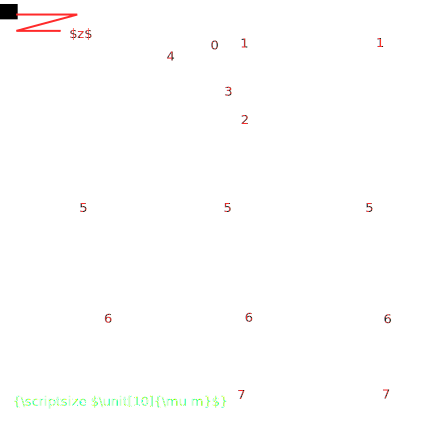
\includegraphics[width=8cm]{m_wf}
    \svginput{.6}{m_wf}
    \svginput{.6}{m_sec}
    \caption{{\bf left:} Wide field focus series of a
      three-dimensional distribution of yellow-green beads in agarose
      gel. Sampling in $z$ is $\unit[1]{\mu m}$. {\bf left:}
      Computationally sectioned images of the same sample. The
      corresponding raw images are shown in \figref{fig:m_phase} on
      page \pageref{fig:m_phase}.}
  \label{fig:m_wf}
\end{figure}

In those cases \cma{optical sectioning} it is useful to utilize
structured illumination to separate out-of-focus and in-focus
fluorescence. The mosaic on the right of \figref{fig:m_wf} shows the
computed optical sections from four raw images per slice. The raw
images are displayed in \figref{fig:m_phase} on page
\pageref{fig:m_phase}.  The optical sections contain relatively distinct
vertical reconstruction artifacts. These can be avoided by using the HiLo
reconstruction method which has the additional advantage of only
needing two raw images per slice.

However, \cma{bead localization} the HiLo method needs considerably
more programming. Also, the artifacts have no effect on the localization
precision of the algorithm. For localization, I determine the center of
each bead by finding local maxima after applying a three-dimensional
difference of Gaussian filter (matched to the bead diameter). The
resulting coordinates are depicted in the inlay in \figref{fig:m_ang}.

% \begin{figure}[hbtp]
%   \centering
%   \svginput{.7}{m_sec}
%   \caption{}
%   \label{fig:m_sec}
% \end{figure}

In the next step, each bead is illuminated individually by displaying
a bright disk at the corresponding position on the focal plane SLM,
while the pupil plane SLM displays a mask which prevents
exposure of out-of-focus beads. This mask is calculated automatically
with a raytracer and utilizes the three-dimensional model of the bead
distribution.


\begin{figure}[hbtp]
  \centering
  \svginput{1}{angular-beads}
  \caption{{\bf left inlay:} Coordinates of the beads from
    \figref{fig:m_wf}. {\bf top mosaic:} Camera images with
    spatio-angular illumination of the beads. This is not a focus
    series but an image of each individual bead. {\bf bottom mosaic:}
    Corresponding patterns of the pupil plane SLM.}
  \label{fig:m_ang}
\end{figure}

The eight camera images of the individual beads are shown in the two
top rows in \figref{fig:m_ang}. Unlike \figref{fig:m_wf}, no focal
series is shown. Each image is focused on a single bead. The
corresponding pupil plane SLM masks are shown in the two rows below. I
will briefly describe \cma{description of pupil plane masks} the
construction of the masks using bead 4 as an example. According to the
three-dimensional diagram in the inlay in \figref{fig:m_ang}, bead 4 is
on the edge of the bead distribution. The smallest angle relative to
the optical axis is between the connecting line of bead 4 and
7. Therefore, the single ``shadow'' (indicated with an arrow) in the
pupil plane mask corresponds to bead 7. All other beads would only be
illuminated by light that strikes bead 4 under a larger angle. Bead 6
and maybe bead 5 combine to the second shadow on the periphery of the
pupil.

The \cma{stability} camera images of bead 2 and 7 in
\figref{fig:m_ang} stand out because they are completely dark. The
reason is that the registration between the focal plane SLM and camera
has shifted by a few microns between localizing the beads and their
spatio-angular exposure. This type of error was corrected by removing
rubber feet from the microscope and screwing it directly to the metal
table.

 

A \cma{artifacts} more interesting effect is visible in the camera
image of bead 5. Only the bottom half of the bead is illuminated but
due to fluorescence in the agarose gel, the circular area that is
illuminated by the focal plane SLM is still visible. This effect would
predominantly occur in samples where fluorescent areas are not sharply
defined. As exposures with light from different angles will contain
different contributions of background fluorescence, it is not clear
whether individual sub-images of the spatio-angular microscope can be
joined into a seamless image. The image quality of confocal
microscopes hardly seems achievable by our system. Cells in an embryo can probably
be counted and tracked, but a quantitative measurement of the
fluorescence seems difficult.

I \cma{comparison spatial control and only angular control} imaged the
beads in \figref{fig:m_ang} with both full angles and optimized
angles. The selective illumination of individual beads using
only the focal plane SLM and full angles already reduced the background
fluorescence from other beads and the gel
significantly. Unfortunately, it is not possible to discern any
further improvement with additional angular control.  I think the
fluorescence from out-of-focus beads can not be detected in the presence of photon
shot noise of the fluorescence from the gel. Angular control will
still have a positive effect because out-of-focus beads are not
uselessly exposed --- it is just not possible to measure this in this
particular sample.

\section{Angular illumination and a higher concentration of beads}
In order to measure the influence of angular illumination control
directly, I made another sample with higher concentration of beads in
an agarose gel with significantly less fluorescence.


\begin{figure}[!hbt]
  \centering
  \svginput{.9}{montage-ang}
  \caption{Dense beads in agarose gel {\bf top left:} Wide field image
    of the beads. The target bead is highlighted with a white circle.
    {\bf bottom left:} Target bead is selectively illuminated by the
    focal plane SLM (using all angles).  {\bf right mosaic:} Variation
    of illumination angle. The contrast of out-of-focus beads is
    increased by scaling the values with a factor of 100 compared to
    the two images on the left.}
  \label{fig:montage-ang}
\end{figure}

The images are shown in \figref{fig:montage-ang}. In the wide field
image, I indicate one bead with a white circle. In the other images,
this bead is selectively illuminated using the focal plane SLM white
circle with dashed outline.

For simplicity, I have omitted the raytrace illumination optimization
and just vary a circular window on the pupil plane SLM ($\rho=0.7,
r=0.3$, with the same geometry as in \figref{fig:overview-bleach}~(e)).


In the mosaic on the right side of \figref{fig:montage-ang}, the
intensity is displayed with a factor of $100\times$ compared to the
previous two images. The same scaling is applied to the images of the
mosaic. The intensity of the central bead is clipped. The illumination
cone that moves with the window manifests itself as a change in the
relative intensities of the out-of-focus beads. A difference can be
seen, for example, in the point marked by an arrow in the pictures for
$\theta=30^\circ$ and $\theta=330^\circ$.

\section{Conclusion}
The described experiments demonstrate that the hardware of the
microscope is functioning as intended, although the performance is
impaired by low transmission and long pattern loading times.

Especially for the experiment in section \ref{sec:beads_under}, a lot
of software had to work in conjunction. The mapping between focal
plane SLM and camera has to be established, the beads must be located
and optimal illumination patterns must be found. These algorithms
should work in close combination with the hardware control, so that
the entire experiment can run with as little user interaction as
possible and finish within reasonable time.

% Das Hauptproblem und der groesste Zeitaufwand lag hier vor allem an
% nicht ausreichenden Informationen ueber einige der nicht ersetzbaren,
% alternativlosen Hardwarekomponenten.

%%% Local Variables: 
%%% mode: latex
%%% TeX-master: "kielhorn_memi"
%%% eval: (reftex-mode)
%%% eval: (flyspell-mode)
%%% End: 
